% In this chapter we have reviewed how to find the distance traveled by an object in motion along a line and (for BC students) along a parametrically defined curve in a plane. We've also looked at a broad variety of applications of the definite integral to other situations where definite integrals of rates of change are used to determine accumulated change, using limits of Riemann sums to create the integrals required.


% The aim of these questions is mainly to reinforce how to set up definite integrals, rather than how to integrate or evaluate them. Therefore we encourage using a graphing calculator wherever helpful.

\question
A particle moves along a line in such a way that its position at time $t$ is given by $s=t^{3}-6 t^{2}+9 t+3$. Its direction of motion changes when
\begin{choices}
  \choice $t=1$ only
  \choice $t=2$ only
  \choice $t=3$ only
  \CorrectChoice $t=1$ and $t=3$
  \choice $t=1,2$, and 3
\end{choices}
\begin{solution}
Velocity $v(t)=\dfrac{d s}{d t}=3(t-1)(t-3)$, and changes sign both when $t=1$ and when $t=3$.
\end{solution}

\question
A body moves along a straight line so that its velocity $v$ at time $t$ is given by $v=4 t^{3}+3 t^{2}+5$. The distance the body covers from $t=0$ to $t=2$ equals
\begin{choices}
  \CorrectChoice $34$
  \choice $55$
  \choice $24$
  \choice $44$
  \choice none of these
\end{choices}
\begin{solution}
Since $v>0$ for $0 \leqq t \leqq 2$, the distance is equal to $\int_{0}^{2}\left(4 t^{3}+3 t^{2}+5\right) d t$.
\end{solution}

\question\label{calc08:particle-v}
A particle moves along a line with velocity $v=3 t^{2}-6 t$. The total distance traveled from $t=0$ to $t=3$ equals
\begin{choices}
  \choice $9$
  \choice $4$
  \choice $2$
  \choice $16$
  \CorrectChoice none of these
\end{choices}
\begin{solution}
The answer is $8$. Since the particle reverses direction when $t=2$, and $v>0$ for $t>2$ but $v<0$ for $t<2$, therefore, the total distance is
\[
-\int_{0}^{2}\left(3 t^{2}-6 t\right) d t+\int_{2}^{3}\left(3 t^{2}-6 t\right) d t
\]
\end{solution}



\newpage



\question
The net change in the position of the particle in Question~\ref{calc08:particle-v}
\begin{choices}
  \choice $2$
  \choice $4$
  \choice $9$
  \choice $16$
  \CorrectChoice none of these
\end{choices}
\begin{solution}
$\int_{0}^{3}\left(3 t^{2}-6 t\right) d t=0$, so there is no change in position.
\end{solution}

\question
The acceleration of a particle moving on a straight line is given by $a=\cos t$, and when $t=0$ the particle is at rest. The distance it covers from $t=0$ to $t=2$ is
\begin{choices}
  \choice $\sin 2$
  \CorrectChoice $1-\cos 2$
  \choice $\cos 2$
  \choice $\sin 2-1$
  \choice $-\cos 2$
\end{choices}
\begin{solution}
Since $v=\sin t$ is positive on $0<t \leqq 2$, the distance covered is


\[
\int_{0}^{2} \sin t d t=1-\cos 2
\]


\end{solution}

\question
During the worst $4-\mathrm{hr}$ period of a hurricane the wind velocity, in miles per hour, is given by $v(t)=5 t-t^{2}+100,0 \leqslant t \leqslant 4$. The average wind velocity during this period (in mph) is
\begin{choices}
  \choice $10$
  \choice $100$
  \choice $102$
  \CorrectChoice $104 \dfrac{2}{3}$
  \choice $108 \dfrac{2}{3}$
\end{choices}
\begin{solution}
Average velocity $=\dfrac{1}{4-0} \int_{0}^{4}\left(5 t-t^{2}+100\right) d t=104 \dfrac{2}{3} \mathrm{mph}$.
\end{solution}






\newpage



\question
A car accelerates from 0 to 60 mph in 10 sec , with constant acceleration. (Note that $60 \mathrm{mph}=88 \mathrm{ft} / \mathrm{sec}$.) The acceleration (in $\mathrm{ft} / \mathrm{sec}^{2}$ ) is
\begin{choices}
  \choice $5.3$
  \choice $6$
  \choice $8$
  \CorrectChoice $8.8$
  \choice none of these
\end{choices}
\begin{solution}
The velocity $v$ of the car is linear since its acceleration is constant:


\[
a=\dfrac{d v}{d t}=\dfrac{(60-0) \mathrm{mph}}{10 \mathrm{sec}}=\dfrac{88 \mathrm{ft} / \mathrm{sec}}{10 \mathrm{sec}}=8.8 \mathrm{ft} / \mathrm{sec}^{2}
\]


\end{solution}

\begin{EnvFullwidth}
\textit{In Questions~\ref{calc08:vector-first}--\ref{calc08:vector-last}, the velocity $\mathbf{v}$ of a particle moving on a curve is given, at time $t$, by $\mathbf{v}=t \mathbf{i}-(1-t) \mathbf{j}$. When $t=0$, the particle is at point $(0,1)$.}
\end{EnvFullwidth}

\question\label{calc08:vector-first}
At time $t$ the position vector $\mathbf{R}$ is
\begin{choices}
  \choice $\dfrac{t^{2}}{2} \mathbf{i}-\dfrac{\left(1-t^{2}\right)}{2} \mathbf{j}$
  \choice $\dfrac{t^{2}}{2} \mathbf{i}+\dfrac{(1-t)^{2}}{2} \mathbf{j}$
  \choice $\dfrac{t^{2}}{2} \mathbf{i}+\dfrac{t^{2}-2 t}{2} \mathbf{j}$
  \CorrectChoice $\dfrac{t^{2}}{2} \mathbf{i}+\dfrac{t^{2}-2 t+2}{2} \mathbf{j}$
  \choice $\dfrac{t^{2}}{2} \mathbf{i}+(1-t)^{2} \mathbf{j}$
\end{choices}
\begin{solution}
$\mathbf{v}=\dfrac{d \mathbf{R}}{d t}$, so $\mathbf{R}(t)=\left(\dfrac{t^{2}}{2}+c_{1}\right) \mathbf{i}+\left(\dfrac{t^{2}}{2}-t+c_{2}\right) \mathbf{j}$. Since $\mathbf{R}(0)=(0,1)$, $c_{1}=0$ and $c_{2}=1$.
\end{solution}

\question
The acceleration vector at time $t=2$ is
\begin{choices}
  \CorrectChoice $\mathbf{i}+\mathbf{j}$
  \choice $\mathbf{i}-\mathbf{j}$
  \choice $\mathbf{i}+2 \mathbf{j}$
  \choice $2 \mathbf{i}-\mathbf{j}$
  \choice none of these
\end{choices}
\begin{solution}
$\mathbf{a}=\mathbf{v}^{\prime}(t)=\mathbf{i}+\mathbf{j}$ for all $t$.
\end{solution}



\newpage



\question\label{calc08:vector-last}
The speed of the particle is at a minimum when $t$ equals
\begin{choices}
  \choice $0$
  \CorrectChoice $\dfrac{1}{2}$
  \choice $1$
  \choice $1.5$
  \choice $2$
\end{choices}
\begin{solution}
$\mathrm{v}=t \mathbf{i}+(t-1) \mathbf{j} .|\mathbf{v}|=\sqrt{t^{2}+(t-1)^{2}} ; \dfrac{d|\mathbf{v}|}{d t}=\dfrac{2 t-1}{|\mathbf{v}|} ; \dfrac{d|\mathbf{v}|}{d t}=0$ at $t=\dfrac{1}{2}$.
\end{solution}

\question
A particle moves along a curve in such a way that its position vector and velocity vector are perpendicular at all times. If the particle passes through the point $(4,3)$, then the equation of the curve is
\begin{choices}
  \choice $x^{2}+y^{2}=5$
  \CorrectChoice $x^{2}+y^{2}=25$
  \choice $x^{2}+2 y^{2}=34$
  \choice $x^{2}-y^{2}=7$
  \choice $2 x^{2}-y^{2}=23$
\end{choices}
\begin{solution}
Since $\mathbf{R}=x \mathbf{i}+y \mathbf{j}$, its slope is $\dfrac{y}{x}$; since $\mathbf{v}=\dfrac{d x}{d t} \mathbf{i}+\dfrac{d y}{d t} \mathbf{j}$, its slope is $\dfrac{d y}{d x}$. If $\mathbf{R}$ is perpendicular to $\mathbf{v}$, then $\dfrac{y}{x} \cdot \dfrac{d y}{d x}=-1$, so


\[
\dfrac{y^{2}}{2}=-\dfrac{x^{2}}{2}+C \quad \text { and } \quad x^{2}+y^{2}=k \quad(k>0) .
\]

Since $(4,3)$ is on the curve, the equation must be

\[
x^{2}+y^{2}=25
\]


\end{solution}

\question
The acceleration of an object in motion is given by the vector $\vec{a}(t)=\left(2 t, e^{t}\right)$. If the object's initial velocity was $\vec{v}(0)=(2,0)$, which is the velocity vector at any time $t$ ?
\begin{choices}
  \choice $\vec{v}(t)=\left(t^{2}, e^{t}\right)$
  \choice $\vec{v}(t)=\left(t^{2}, e^{t}+1\right)$
  \choice $\vec{v}(t)=\left(t^{2}+2, e^{t}\right)$
  \CorrectChoice $\vec{v}(t)=\left(t^{2}+2, e^{t}-1\right)$
  \choice $\vec{v}(t)=\left(2, e^{t}-1\right)$
\end{choices}
\begin{solution}
$\vec{v}(t)=\left(t^{2}+c_{1}, e^{t}+c_{2}\right)$; since $\vec{v}(0)=(2,0), 0^{2}+c_{1}=2$ and $e^{0}+c_{2}=0$; hence $c_{1}=2$ and $c_{2}=-1$.
\end{solution}



\newpage



\question
The velocity of an object is given by $\vec{v}(t)=(3 \sqrt{t}, 4)$. If this object is at the origin when $t=1$, where was it at $t=0$ ?
\begin{choices}
  \choice $(-3,-4)$
  \CorrectChoice $(-2,-4)$
  \choice $(2,4)$
  \choice $\left(\dfrac{3}{2}, 0\right)$
  \choice $\left(-\dfrac{3}{2}, 0\right)$
\end{choices}
\begin{solution}
The object's position is given by $x(t)=2 t^{\dfrac{3}{2}}+c_{1}, y(t)=4 t+c_{2}$. Since the object was at the origin at $t=1,2 \cdot 1^{\dfrac{3}{2}}+c_{1}=0$ and $4 \cdot 1+c_{2}=0$, making the position $x(t)=2 t^{\dfrac{3}{2}}-2, y(t)=4 t-4$. When $t=0, x(0)=-2, y(0)=-4$.
\end{solution}

\question
Suppose the current world population is 6 billion and the population $t \mathrm{yr}$ from now is estimated to be $P(t)=6 e^{0.024 t}$. On the basis of this supposition, the average population of the world, in billions, over the next 25 yr will be approximately
\begin{choices}
  \choice $6.75$
  \choice $7.2$
  \choice $7.8$
  \CorrectChoice $8.2$
  \choice $9.0$
\end{choices}
\begin{solution}
$\dfrac{1}{25-0} \int_{0}^{25} P(t) d t=\dfrac{1}{25} \int_{0}^{25} 6 e^{0.024 t} \simeq 8.2$ (billion people).
\end{solution}

\question
If a quantity $Q(t)$ is growing at the rate of $5 \%$ per year and $Q$ now equals $Q_{0}$, then in $t \mathrm{yr} Q$ will equal
\begin{choices}
  \choice $Q_{0}(1.05 t)$
  \CorrectChoice $Q_{0}(1.05)^{t}$
  \choice $Q_{0} e^{0.05 t}$
  \choice $Q_{0} e^{0.045 t}$
  \choice none of these
\end{choices}
\begin{solution}
"A quantity growing at the rate of $5 \%$ per year" means that after 1 yr the quantity $Q_{0}$ will have grown to $1.05 Q_{0}$, after 2 yr to $1.05\left(1.05 Q_{0}\right), \ldots$, after $t \mathrm{yr}$ to $(1.05)^{t} \cdot Q_{0}$.
\end{solution}



\newpage



\question
A beach opens at 8 A.M. and people arrive at a rate of $R(t)=10+40 t$ people per hour, where $t$ represents the number of hours the beach has been open. Assuming no one leaves before noon, at what time will there be 100 people there?
\begin{choices}
  \choice $9: 45$
  \CorrectChoice 10:00
  \choice $10: 15$
  \choice $10: 30$
  \choice $10: 45$
\end{choices}
\begin{solution}
We want the accumulated number of people to be 100 :


\[
\begin{aligned}
\int_{0}^{h}(10+40 t) d t & =100 \\
\left.\left(10 t+20 t^{2}\right)\right|_{0} ^{h} & =100 \\
20 h^{2}+10 h-100 & =0 \\
10(2 h+5)(h-2) & =0
\end{aligned}
\]

This occurs at $h=2$ hours after 8 A.M.
\end{solution}

\question
A stone is thrown upward from the ground with an initial velocity of $96 \mathrm{ft} / \mathrm{sec}$. Its average velocity (given that $a(t)=-32 \mathrm{ft} / \mathrm{sec}^{2}$ ) during the first 2 sec is
\begin{choices}
  \choice $16 \mathrm{ft} / \mathrm{sec}$
  \choice $32 \mathrm{ft} / \mathrm{sec}$
  \CorrectChoice $64 \mathrm{ft} / \mathrm{sec}$
  \choice $80 \mathrm{ft} / \mathrm{sec}$
  \choice $96 \mathrm{ft} / \mathrm{sec}$
\end{choices}
\begin{solution}
(C) Average velocity $=\dfrac{1}{2-0} \int_{0}^{2}(-32 t+96) d t=64 \mathrm{ft} / \mathrm{sec}$.
\end{solution}

\question
Suppose the amount of a drug in a patient's bloodstream $t \mathrm{hr}$ after intravenous administration is $30 /(t+1)^{2} \mathrm{mg}$. The average amount in the bloodstream during the first 4 hr is
\begin{choices}
  \CorrectChoice 6.0 mg
  \choice 11.0 mg
  \choice 16.6 mg
  \choice 24.0 mg
  \choice none of these
\end{choices}
\begin{solution}
(A) Average volume $=\dfrac{1}{4-0} \int_{0}^{4} \dfrac{30}{(t+1)^{2}} d t \simeq 6 \mathrm{mg}$.
\end{solution}



\newpage



\question
A rumor spreads through a town at the rate of $\left(t^{2}+10 t\right)$ new people per day. Approximately how many people hear the rumor during the second week after it was first heard?
\begin{choices}
  \CorrectChoice $1535$
  \choice $1894$
  \choice $2000$
  \choice $2219$
  \choice none of these
\end{choices}
\begin{solution}
(A) The number of new people who hear the rumor during the second week is

\[
\int_{7}^{14}\left(t^{2}+10 t\right) d t \simeq 1535
\]

Be careful with the units! The answer is the total change, of course, in $F(t)$ from $t=7$ to $t=14$ days, where $F^{\prime}(t)=t^{2}+10 t$.
\end{solution}

\question\label{calc08:oil-leak}
Oil is leaking from a tanker at the rate of $1000 e^{-0.3 t} \mathrm{gal} / \mathrm{hr}$, where $t$ is given in hours. A general Riemann sum for the amount of oil that leaks out in the next 8 hr , where the interval $[0,8]$ has been partitioned into $n$ subintervals, is
\begin{choices}
  \choice $\sum_{k=1}^{n} e^{-0.3 t_{k}} \Delta t$
  \choice $\lim\limits_{n \to \infty} \sum_{k=1}^{n} e^{-0.3 t_{k}} \Delta t$
  \choice $\lim\limits_{n \to \infty} \sum_{k=1}^{n} 1000 e^{-0.3 t_{k}} \Delta t$
  \CorrectChoice $\sum_{k=1}^{n} 1000 e^{-0.3 t_{k}} \Delta t$
  \choice $1000 \sum_{k=1}^{n} e^{0.3 t_{k}} \Delta t$
\end{choices}
\begin{solution}
(D) After partitioning $[0,8]$ into $n$ subintervals, we approximate the amount of oil leaking in a typical subinterval of duration $\Delta t$ : it is

\[
1000 e^{-0.3 t_{k}} \Delta t \mathrm{gal} / \mathrm{hr} \times \mathrm{hr} .
\]

For the general Riemann sum we can choose any point in a subinterval, not necessarily the leftmost or rightmost; we've denoted this arbitrary choice by the subscript $k$. This sum now adds all $n$ of the small quantities of oil (in gallons).
\end{solution}

\question
In Question~\ref{calc08:oil-leak}, the total number of gallons of oil that will leak out during the next 8 hr is approximately
\begin{choices}
  \choice $1271$
  \CorrectChoice $3031$
  \choice $3161$
  \choice $4323$
  \choice $11{,}023$
\end{choices}
\begin{solution}
(B) Total gallons $=\lim\limits_{n \to \infty} \sum_{k=1}^{n} 1000 e^{-0.3 t_{k}} \Delta t=\int_{0}^{8} 1000 e^{-0.3 t} d t \approx 3031$.
\end{solution}



\newpage



\question
Assume that the density of vehicles (number per mile) during morning rush hour, for the $20-\mathrm{mi}$ stretch along the New York State Thruway southbound from the Tappan Zee Bridge, is given by $f(x)$, where $x$ is the distance, in miles, south of the bridge. Which of the following gives the number of vehicles (on this $20-\mathrm{mi}$ stretch) from the bridge to a point $x \mathrm{mi}$ south of the bridge?
\begin{choices}
  \CorrectChoice $\int_{0}^{x} f(t) d t$
  \choice $\int_{x}^{20} f(t) d t$
  \choice $\int_{0}^{20} f(x) d x$
  \choice $\sum_{k=1}^{n} f\left(x_{k}\right) \Delta x$ (where the 20 -mi stretch has been partitioned into $n$ equal subintervals)
  \choice none of these
\end{choices}
\begin{solution}
(A) Be careful! The number of cars is to be measured over a distance of $x$ (not $20) \mathrm{mi}$. The answer to the question is a function, not a number. Note that choice (C) gives the total number of cars on the entire $20-\mathrm{mi}$ stretch.
\end{solution}

\question
The center of a city that we will assume is circular is on a straight highway. The radius of the city is 3 mi . The density of the population, in thousands of people per square mile, is given approximately by $f(r)=12-2 r$ at a distance $r$ mi from the highway. The population of the city is given by the integral
\begin{choices}
  \choice $\int_{0}^{3}(12-2 r) d r$
  \choice $2 \int_{0}^{3}(12-2 r) \sqrt{9-r^{2}} d r$
  \CorrectChoice $4 \int_{0}^{3}(12-2 r) \sqrt{9-r^{2}} d r$
  \choice $\int_{0}^{3} 2 \pi r(12-2 r) d r$
  \choice $2 \int_{0}^{3} 2 \pi r(12-2 r) d r$
\end{choices}
\begin{solution}
(C) Since the strip of the city shown in the figure is at a distance $r$ mi from the highway, it is $2 \sqrt{9-r^{2}}$ mi long and its area is $2 \sqrt{9-r^{2}} \Delta r$. The strip's population is approximately $2(12-2 r) \sqrt{9-r^{2}} \Delta r$. The total population of the entire city is twice the integral $2 \int_{0}^{3}(12-2 r) \sqrt{9-r^{2}} d r$ as it includes both halves of the city.
\begin{center}
  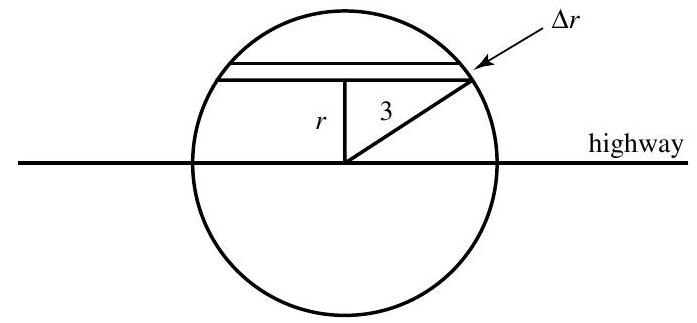
\includegraphics[width=0.50\linewidth]{calculus/images/511798ce-a7b4-495d-9fd4-3cff1fa82426-08_323_697_1178_742.jpg}
\end{center}
\end{solution}



\newpage



\question
The population density of Winnipeg, which is located in the middle of the Canadian prairie, drops dramatically as distance from the center of town increases. This is shown in the following table:

\begin{center}
\begin{tabular}{c|cccccc}
$x$ (distance in mi) & 0 & 2 & 4 & 6 & 8 & 10 \\
\hline
density (people/mi$^2$) & 50 & 45 & 40 & 30 & 15 & 5 \\
\end{tabular}
\end{center}

Using a Riemann sum, we can calculate the population living within a $10-\mathrm{mi}$ radius of the center to be approximately
\begin{choices}
  \choice $608{,}500$
  \choice $650{,}000$
  \CorrectChoice $691{,}200$
  \choice $702{,}000$
  \choice $850{,}000$
\end{choices}
\begin{solution}
(C)
\begin{center}
  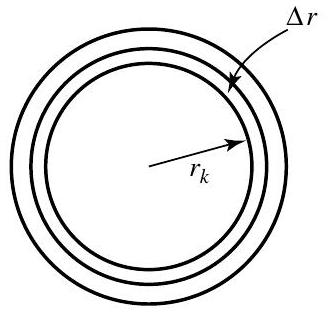
\includegraphics[width=0.40\linewidth]{calculus/images/511798ce-a7b4-495d-9fd4-3cff1fa82426-08_314_328_1563_1011.jpg}
\end{center}
\begin{center}
  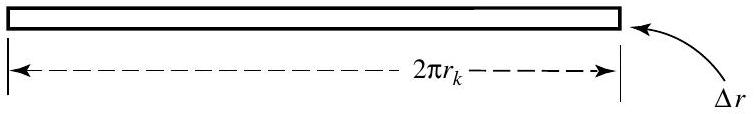
\includegraphics[width=0.40\linewidth]{calculus/images/511798ce-a7b4-495d-9fd4-3cff1fa82426-08_114_755_1902_735.jpg}
\end{center}

The population equals $\sum$ (area  density). We partition the interval $[0,10]$ along a radius from the center of town into 5 equal subintervals each of width $\Delta r=2 \mathrm{mi}$. We will divide Winnipeg into 5 rings. Each has area equal to (circumference  width), so the area is $2 \pi r_{k} \Delta r$ or $4 \pi r_{k}$. The population in the ring is

\[
\left(4 \pi r_{k}\right) \cdot\left(\text { density at } r_{k}\right)=4 \pi r_{k} \cdot f\left(r_{k}\right) .
\]

A Riemann sum, using left-hand values, is $4 \pi \cdot 0 \cdot 50+4 \pi \cdot 2 \cdot 45+ 4 \pi \cdot 4 \cdot 40+4 \pi \cdot 6 \cdot 30+4 \pi \cdot 8 \cdot 15=4 \pi(90+160+180+120) \simeq 6912$ hundred people-or about 691,200 people.
\end{solution}


\newpage




\question
If a factory continuously dumps pollutants into a river at the rate of $\dfrac{\sqrt{t}}{180}$ tons per day, then the amount dumped after 7 weeks is approximately
\begin{choices}
  \choice 0.07 ton
  \choice 0.90 ton
  \choice 1.55 tons
  \choice 1.9 tons
  \CorrectChoice 1.27 tons
\end{choices}
\begin{solution}
(E) The total amount dumped after 7 weeks is

\[
\int_{0}^{49} \dfrac{\sqrt{t}}{180} d t \simeq 1.27 \text { tons }
\]


\end{solution}

\question
A roast at $160^{\circ} \mathrm{F}$ is put into a refrigerator whose temperature is $45^{\circ} \mathrm{F}$. The temperature of the roast is cooling at time $t$ at the rate of $\left(-9 e^{-0.08 t}\right)^{\circ} \mathrm{F}$ per minute. The temperature, to the nearest degree F , of the roast 20 min after it is put in the refrigerator is
\begin{choices}
  \choice $45^{\circ}$
  \CorrectChoice $70^{\circ}$
  \choice $81^{\circ}$
  \choice $90^{\circ}$
  \choice $115^{\circ}$
\end{choices}
\begin{solution}
The total change in temperature of the roast 20 min after it is put in the refrigerator is
\[
\int_{0}^{20}-9 e^{-0.08 t} d t \quad \text { or } \quad-89.7^{\circ} \mathrm{F}
\]
Since its temperature was $160^{\circ} \mathrm{F}$ when placed in the refrigerator, then 20 min later it is $(160-89.7)^{\circ} \mathrm{F}$ or about $70^{\circ} \mathrm{F}$. Note that the temperature of the refrigerator ( $45^{\circ} \mathrm{F}$ ) is not used in answering the question because it is already "built into" the cooling rate.
\end{solution}





\newpage




\question
How long will it take to release 9 tons of pollutant if the rate at which pollutant is being released is $t e^{-0.3 t}$ tons per week?
\begin{choices}
  \CorrectChoice 10.2 weeks
  \choice 11.0 weeks
  \choice 12.1 weeks
  \choice 12.9 weeks
  \choice none of these
\end{choices}
\begin{solution}
(A) Let $T$ be the number of weeks required to release 9 tons. We can use parts to integrate $\int_{0}^{T} t e^{-0.3 t} d t$, then substitute the limits. We must then set the resulting expression equal to 9 and solve for $T$. A faster, less painful alternative is to use a graphing calculator to solve the equation

\[
\int_{0}^{T} t e^{-0.3 t} d t=9
\]

The answer is about 10.2 weeks.
\end{solution}

\question
If you deposit $\$ 1000$ today at $8 \%$ interest compounded continuously, it will grow at the rate of $80 e^{0.08 t}$ dollars per year. In 6 years it will be worth (in dollars)
\begin{choices}
  \choice $616.07$
  \choice $1129.29$
  \choice $1292.86$
  \CorrectChoice $1616.07$
  \choice $6160.74$
\end{choices}
\begin{solution}
(D) The amount by which your investment of $\$ 1000$ today will increase in 6 yr is $\int_{0}^{6} 80 e^{0.08 t} d t$ or $\$ 616.07$, so it will be worth $\$(1000+616.07)$.
Note: $1000 e^{0.08(6)}=\$ 1616.07$.
\end{solution}

\question
The average area, in square inches, of all circles with radii between 2 and 5 in. is
\begin{choices}
  \choice $7 \pi$
  \choice $11 \pi$
  \CorrectChoice $13 \pi$
  \choice $\dfrac{29 \pi}{2}$
  \choice $17 \pi$
\end{choices}
\begin{solution}
(C) Average area $=\dfrac{1}{5-2} \int_{2}^{5} \pi x^{2} d x=\dfrac{\pi}{3}\left(\dfrac{125-8}{3}\right)=13 \pi \mathrm{in}^{2}$.
\end{solution}



\newpage




\question
What is the exact total area bounded by the curve $f(x)=x^{3}-4 x^{2}+3 x$ and the $x$-axis?
\begin{choices}
  \choice $-2.25$
  \choice $2.25$
  \choice $3$
  \CorrectChoice $3.083$
  \choice none of these
\end{choices}
\begin{solution}
(D) Note that the curve is above the $x$-axis on $[0,1]$, but below on $[1,3]$, and that the areas for $x<0$ and $x>3$ are unbounded.
\begin{center}
  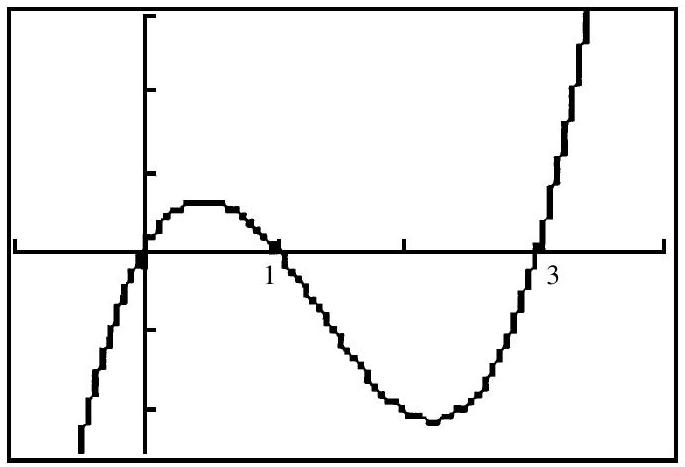
\includegraphics[width=0.50\linewidth]{calculus/images/511798ce-a7b4-495d-9fd4-3cff1fa82426-09_467_685_1971_1011.jpg}
\end{center}Using the calculator, we get

\[
\int_{0}^{3}\left|x^{3}-4 x^{2}+3 x\right| d x \approx 3.083
\]


\end{solution}

\question
Water is leaking from a tank at the rate of $\left(-0.1 t^{2}-0.3 t+2\right) \mathrm{gal} / \mathrm{hr}$. The total amount, in gallons, that will leak out in the next 3 hr is approximately
\begin{choices}
  \choice $1.00$
  \choice $2.08$
  \choice $3.13$
  \choice $3.48$
  \CorrectChoice $3.75$
\end{choices}
\begin{solution}
The FTC yields total change:
\[
\int_{0}^{3}\left(-0.1 t^{2}-0.3 t+2\right) d t \simeq 3.75 \mathrm{gal}
\]
\end{solution}



\newpage




\question
A bacterial culture is growing at the rate of $1000 e^{0.03 t}$ bacteria in $t$ hr. The total increase in bacterial population during the second hour is approximately
\begin{choices}
  \choice $46$
  \choice $956$
  \CorrectChoice $1046$
  \choice $1061$
  \choice $2046$
\end{choices}
\begin{solution}
The total change (increase) in population during the second hour is given by $\int_{1}^{2} 1000 e^{0.03 t} d t$. The answer is 1046 .
\end{solution}

\question
An 18 -wheeler traveling at speed $v$ mph gets about $(4+0.01 v) \mathrm{mpg}$ (miles per gallon) of diesel fuel. If its speed is $80 \dfrac{t+1}{t+2} \mathrm{mph}$ at time $t$, then the amount, in gallons, of diesel fuel used during the first 2 hr is approximately
\begin{choices}
  \choice $20$
  \choice $21.5$
  \CorrectChoice $23.1$
  \choice $24$
  \choice $25$
\end{choices}
\begin{solution}
We partition $[0,2]$ into $n$ equal subintervals each of time $\Delta t \mathrm{hr}$. Since the 18 -wheeler gets $(4+0.01 v) \mathrm{mi} / \mathrm{gal}$ of diesel, it uses $\dfrac{1}{4+0.01 v} \mathrm{gal} / \mathrm{mi}$.
Since it covers $v \cdot \Delta t$ mi during $\Delta t \mathrm{hr}$, it uses $\dfrac{1}{4+0.01 v} \cdot v \cdot \Delta t$ gal in $\Delta t \mathrm{hr}$.
Since $v=80 \dfrac{t+1}{t+2}$, we see that the diesel fuel used in the first 2 hr is


\[
\int_{0}^{2} \dfrac{80 \cdot \dfrac{t+1}{t+2}}{4+(0.01) \cdot\left(80 \cdot \dfrac{t+1}{t+2}\right)} d t=\int_{0}^{2} \dfrac{80(t+1)}{4.8 t+8.8} d t \simeq 23.1 \mathrm{gal}
\]
\end{solution}
